\documentclass{../UTNetLabFa}

\title{کلیات شبکه و پشته‌ی \textLR{TCP-IP}}


\begin{document}

% \tableofcontents
% \listoffigures
% \listoftables
% \lstlistoflistings
%\listofcodes
\pagebreak

\part{تمرین های رابط شبکه}
تمرین های زیر از توپولوژی شبکه یک قطعه استفاده می کند که در شکل 1.0 نشان داده شده است.
	{
		\selectlanguage{english}
		\begin{center}
			\begin{minipage}{0.48\textwidth}
				\begin{flushleft}
					\begin{table}[H]
						\caption{The IP addresses of the hosts (Table~1.2)}
						\centering
						\begin{tabular}{ c c c }
							\hline \hline
							Host & IP Address & Subnet Mask \\
							\hline 
							h0 & 128.238.66.100 & 255.255.255.0 \\
							h1 & 128.238.66.101 & 255.255.255.0 \\
							h2 & 128.238.66.102 & 255.255.255.0 \\
							h3 & 128.238.66.103 & 255.255.255.0 \\
							h4 & 128.238.66.104 & 255.255.255.0 \\
							h5 & 128.238.66.105 & 255.255.255.0 \\
							h6 & 128.238.66.106 & 255.255.255.0 \\
							h7 & 128.238.66.107 & 255.255.255.0 \\
							\hline \hline
							\end{tabular}
					\end{table}
				\end{flushleft}
			\end{minipage}
			\begin{minipage}{0.48\textwidth}
				\begin{flushright}
					\begin{figure}[H]
						\centering
						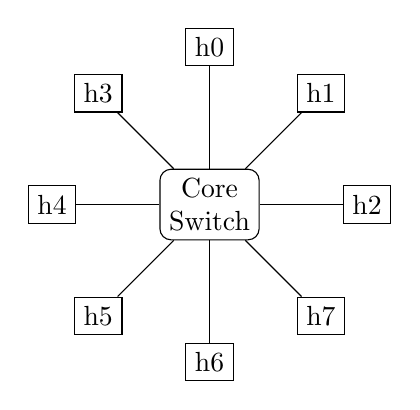
\begin{tikzpicture}
							\node[draw,align=center,rounded corners] (s) at (0,0){Core\\Switch};
							\node[draw] (h0) at (0,2){h0};
							\node[draw] (h1) at ({sqrt(2)},{sqrt(2)}){h1};
							\node[draw] (h2) at (2,0){h2};
							\node[draw] (h3) at (-{sqrt(2)},{sqrt(2)}){h3};
							\node[draw] (h4) at (-2,0){h4};
							\node[draw] (h5) at (-{sqrt(2)},-{sqrt(2)}){h5};
							\node[draw] (h6) at (0,-2){h6};
							\node[draw] (h7) at ({sqrt(2)},-{sqrt(2)}){h7};
						
							\draw (h0) -- (s);
							\draw (h1) -- (s);
							\draw (h2) -- (s);
							\draw (h3) -- (s);
							\draw (h4) -- (s);
							\draw (h5) -- (s);
							\draw (h6) -- (s);
							\draw (h7) -- (s);
						\end{tikzpicture}
						\caption{A single segment network (Figure~1.3)}\label{fig:1.3}
					\end{figure}
				\end{flushright}
			\end{minipage}
		\end{center}
	}

	\section{رابط های شبکه}
	از دستور \textLR{ifconfig -a} استفاده کنید تا اطلاعات مربوط به رابط‌های شبکه در هاست شما نشان داده شود. آدرس آی‌پی و \mbox{\textLR{net mask}} دستگاه خود را بیابید.
	
		\begin{report}
			\item هاست چه تعداد رابط شبکه دارد؟ تمام رابط‌های یافت شده را به همراه نام آنها لیست کنید و عملکرد هر یک را به طور خلاصه توضیح دهید.
			\item \textLR{MTU} هر کدام از رابط‌های هاست شما چیست؟
			\item 	آیا شبکه \textLR{subnet} شده است؟ دلیل جواب خود را بیان کنید. 
		\end{report}
	


	\section{دامپ هاست محلی}
	 مادامی که دستور \textLR{\textbf{tcpdump host} \textit{your-host}} در حال اجرا بر روی یک \mbox{\textLR{command window}} است، دستور \textLR{\textbf{ping 127.0.0.1}} را در یک \mbox{\textLR{command window}} دیگر اجرا کنید.

		\begin{report}
			\item با توجه به خروجی دستور \textLR{\textbf{ping}} ، آیا رابط \textLR{127.0.0.1} روشن است؟
			\item آیا می‌توانید در خروجی دستور \textLR{\textbf{tcpdump}} هر پیام \textLR{ICMP} که از هاست شما ارسال می شود را   ببینید؟ چرا؟
	
		\end{report}
	
	\section{آمار شبکه}
	
	با استفاده از دستور \textLR{\textbf{netstat -ie}} ، آمار را از همه‌ی هاست‌های روی شبکه جمع آوری کنید. از آنجایی که ما از یک نام‌کاربری و رمزعبور یکسان استفاده می‌کنیم، می‌توانیم به سایر \textLR{workstation} ها \textLR{\textbf{telnet}} بزنیم و دستور \textLR{\textbf{netstat -ie}} را روی آن اجرا کنیم.

	خروجی های دستور \textLR{\textbf{netstat -ie}} را ذخیره کنید.

	اگر مقدار زیادی پکت‌های خروجی را در نتایج \textLR{\textbf{netstat}} نمی‌بینید، احتمالا دستگاه به تازگی شروع به کار کرده است.
	شما بهتر است این آزمایش را بعدا انجام دهید، یا از دستور \textLR{\textbf{sock}} زیر استفاده کنید تا مقداری ترافیک شبکه تولید شود:

	
\textLR{\textbf{socket -u -i -n200} \textit{remote-host} \textbf{echo}}
	
	\begin{report}
		\item میانگین نرخ برخورد بر روی همه هاست‌هایی که در مجموعه‌ی آمارهای جمع شده در این تمرین هستند را محاسبه کنید.		
	\end{report}
	
	
\part{تمرین های \textLR{ARP}}
	در آزمایش های زیر، ما باید جدول \textLR{ARP} و عملکرد \textLR{ARP} بر روی هاست را بررسی کنیم، که شامل دو مورد جالب است: \mbox{\textLR{proxy ARP}} و \mbox{\textLR{gratuitous ARP}}. شما ممکن است نیاز داشته باشید که آدرس \textLR{MAC} رابط‌های هاست و \textLR{router} را از مدرس آزمایشگاه بپرسید. سپس آدرس‌ \textLR{MAC} ها را در جدول الف.۱ و جدول الف.۲ در ضمیمه یادداشت کنید. شما به این آدرس \textLR{MAC} ها برای تمرین ها و گزارش آزمایشگاه نیاز دارید.
	\section{جدول \textLR{ARP}}
		از \textLR{\textbf{arp -a}} استفاده کنید تا کل جدول \textLR{ARP} را ببینید. مشاهده کنید که همه آدرس آی‌پی های نمایان شده در یک \textLR{subnet} یکسان هستند. 
		
		اگر متوجه شدید که همه هاست‌های \textLR{remote} در جدول \textLR{ARP} هاست شما وجود دارند، احتیاج به حذف یک هاست \textLR{remote} (بجز هاست خودتان) از جدول با استفاده از دستور \textLR{\textbf{arp -d} \textit{remote-host}} دارید.
		
		جدول \textLR{ARP} را برای گزارش آزمایش خود ذخیره کنید.
		
		مادامی که دستور \textLR{\textbf{tcpdump -en \# -x for see hex dump }} در حال اجرا است، یک هاست \textLR{remote} را که در جدول \textLR{ARP} هاست شما نیست \textLR{\textbf{ping}} کنید. سپس برنامه \textLR{\textbf{ping}} را متوقف کنید.
		
		شما می‌توانید دستور \textLR{\textbf{wireshark \&}} را جهت ضبط شبکه اجرا کنید.
		
		چند خط اول ردیابی بسته‌ها را مشاهده کنید تا ببینید چگونه از \textLR{ARP} برای حل آدرس آی‌پی استفاده می شود.
		
		دستور \textLR{\textbf{arp -a}} را اجرا کنید تا ببینید یک ردیف جدید به جدول \textLR{ARP} هاست شما اضافه شده است. جدول \textLR{ARP} جدید را برای گزارش آزمایشگاه خود ذخیره کنید.
		بسته درخواست \textLR{ARP} و بسته جواب \textLR{ARP} را در پنجره \textLR{wireshark} علامت بزنید. سپس به منوی \textLR{File} رفته و گزینه \textLR{Print...} را جهت چاپ بسته‌های انتخاب شده برای گزارش آزمایشگاه خود انتخاب کنید. (تمرین ۶ فصل اول را ببینید).
	
	\begin{report}
		\item
		با توجه به خروجی ذخیره شده \textLR{\textbf{tcpdump}} توضیح دهید که \textLR{ARP} چگونه عمل می کند؟ 
		\item فرمت یک درخواست ضبط شده \textLR{ARP} و جواب آنرا به همراه فیلد ها و مقادیر آنها رسم کنید.
		\item در یک درخواست \textLR{ARP} ، آی‌پی آدرس مقصد چیست؟
		\item در لایه \textLR{MAC} ، آدرس \textLR{Ethernet} مقصدِ فریم ای که درخواست \textLR{ARP} را حمل می کند، چیست؟
		\item فیلد نوع \textLR{frame} در \textLR{Ethernet frame} چیست ؟	
		\item چه کسی جواب \textLR{ARP} را ارسال می کند؟
	\end{report}
	
	\section{\textLR{ARP timeout}}
	
	مادامی که دستور \textLR{\textbf{tcpdump host} \textit{your-host}} در حال اجرا جهت ضبط کردن ترافیک دستگاه شما می باشد، دستور \mbox{\textLR{\textbf{telnet 128.238.66.200}}} را اجرا کنید.
	
	توجه داشته باشید که هیچ هاست‌ای با این آدرس آی‌پی در پیکربندی فعلی شبکه آزمایشگاه موجود نیست.
	
	چند بسته اولیه در خروجی \textLR{\textbf{tcpdump}} را جهت گزارش آزمایشگاه ذخیره کنید.
	
	بعد از دریافت خروجی مورد نیاز، نشست \textLR{\textbf{telnet}} را قطع کنید.
	
	\begin{report}
		\item
		 	از خروجی ذخیره شده \textLR{\textbf{tcpdump}} ، چگونگی رخ دادن \textLR{ARP timeout} و ارسال مجدد آن را شرح دهید. 
		 \item 
		 چند بار تلاش برای حل کردن آی‌پی آدرسی که ناموجود است، رخ داد؟

	\end{report}

	\section{\textLR{ARP proxy}}
	
	توپولوژی شبکه‌ای که برای این تمرین \textLR{ARP proxy} استفاده شده است، در شکل ۲.۹ نشان داده شده است. ما گروه را به دو \textLR{subnet} که توسط یک \textLR{router} به هم متصل اند، تقسیم خواهیم کرد. آی‌پی آدرس ها و \mbox{\textLR{network mask}} های هاست‌ها در شکل ۲.۹ داده شده است. آدرس آی‌پی و \mbox{\textLR{network mask}} هاست خود را بر این اساس تنظیم کنید (بخش ۲.۳.۲ را ببینید). آدرس آی‌پی و \mbox{\textLR{network mask}} مربوط به رابط‌های \textLR{Router4} مشابه تنظیمات پیشفرض شان هستند. توجه کنید که \mbox{\textLR{network mask}} هاست‌های شبکه \textLR{128.238.65.0} برابر \textLR{255.255.0.0} است.
	
	آی‌پی هر شبکه را با دستورات زیر در هاست‌ها تنظیم کنید:
	
	\begin{enumerate}
		\item \textLR{ifconfig eth0 x.x.x.x/mask}
		\item \textLR{route add default gw x.x.x.x}
	\end{enumerate}
	
	سپس ما عملکرد \textLR{proxy ARP} را بر روی رابط \textLR{ethernet1} مربوط به \textLR{Router4} فعال می کنیم.
	
	\begin{enumerate}
		\item 
			به \textLR{Router4} تلنت کنید:  \textLR{telnet 128.238.64.4}   ( \# در \textLR{GNS3} بر روی \textLR{Router} راست کلیک کنید و یک کنسول باز کنید)
		\item
		به \textLR{router} لاگین کنید، کلمه \textLR{enable} را تایپ کنید تا وارد حالت \textLR{Privileged EXEC} شوید.
		\item
		با تایپ کردن \textLR{config term} به حالت \textLR{Global Configuration} وارد شوید.
		\item
		سپس خطوط زیر را برای هر رابط تایپ کنید:

			\begin{itemize}
				\item \textLR{\textbf{interface f0/0}}  ( \# برای یکی دیگه \textLR{f0/1} بزنید)
				\item \textLR{\textbf{ip addr x.x.x.x 255.255.255.0}}
				\item \textLR{\textbf{no shut}}
				\item \textLR{\textbf{ip proxy-arp}}
				\item \textLR{Ctrl-Z}
				\item \textLR{\textbf{wr}}
			\end{itemize}
	\end{enumerate}

	اکنون رابط \textLR{ethernet1} در \textLR{Router4} می تواند \textLR{proxy ARP} را برای هاست های سابنت \textLR{128.238.64.0} اجرا کند.
	
	دستور \textLR{\textbf{tcpdump -enx}} را بر روی همه‌ی هاست‌ها اجرا کنید.
	
	سپس صبر کنید تا هاست‌های مربوط به سابنت \textLR{128.238.65.0} ، دیتاگرام‌های \textLR{UDP} را به هاست‌های مربوط به سابنت \textLR{128.238.64.0} ارسال کنند.
	
	برای مثال دستور زیر را در هاست \textLR{guchi} وارد کنید:
	
\textLR{\textbf{socket -i -u -n1 -w1000} \textit{Host-in-64.0-subnet} \textbf{echo}}

	وقتی بر روی همه هاست‌های سابنت \textLR{128.238.64.0} انجام دادید، خروجی \textLR{\textbf{tcpdump}} را برای گزارش خود ذخیره کنید.
	
	دستور \textLR{\textbf{arp -a}} را برای نمایش جدول \textLR{ARP} جدید در هاست خود اجرا کنید. خروجی آن را برای گزارش خود ذخیره کنید.
	
	پس از اینکه مدرس آزمایشگاه شبکه را به حالت \textLR{single subnet} بازگرداند (شکل ۱.۳ را ببینید)، آدرس آی‌پی و \textLR{network mask} رابط هاست خود را به مقادیر پیشفرض آن‌ها که در در جدول ۱.۳ آمده است، تغییر دهید.
	
	اطلاعات ذخیره شده در این تمرین را با یک دانشجوی دیگر که در یک سابنت دیگر کار می‌کند، مبادله کنید.
	
	{
		\selectlanguage{english}
		\begin{figure}[H]
			\centering
				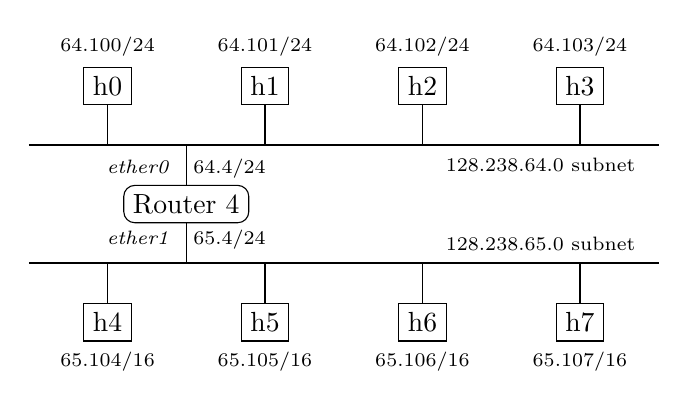
\begin{tikzpicture}
					\draw (0*2,3) node[draw,fill=white] (h0) {h0} -- +(0,-0.75) +(0,+0.5) node {\scriptsize 64.100/24};
					\draw (1*2,3) node[draw,fill=white] (h1) {h1} -- +(0,-0.75) +(0,+0.5) node {\scriptsize 64.101/24};
					\draw (2*2,3) node[draw,fill=white] (h2) {h2} -- +(0,-0.75) +(0,+0.5) node {\scriptsize 64.102/24};
					\draw (3*2,3) node[draw,fill=white] (h3) {h3} -- +(0,-0.75) +(0,+0.5) node {\scriptsize 64.103/24};
					\draw (0*2,0) node[draw,fill=white] (h4) {h4} -- +(0,+0.75) +(0,-0.5) node {\scriptsize 65.104/16};
					\draw (1*2,0) node[draw,fill=white] (h5) {h5} -- +(0,+0.75) +(0,-0.5) node {\scriptsize 65.105/16};
					\draw (2*2,0) node[draw,fill=white] (h6) {h6} -- +(0,+0.75) +(0,-0.5) node {\scriptsize 65.106/16};
					\draw (3*2,0) node[draw,fill=white] (h7) {h7} -- +(0,+0.75) +(0,-0.5) node {\scriptsize 65.107/16};
					\draw (0.5*2,1.5) node[draw,rounded corners,fill=white] (r4) {Router 4}
						-- +(0,+0.75) +(0,+0.45) node {\scriptsize\textit{ether0}\quad 64.4/24}
						-- +(0,-0.75) +(0,-0.45) node {\scriptsize\textit{ether1}\quad 65.4/24}
					;
					\draw[thick] (-1,0.75) -- +({(3+1)*2},0);
					\draw[thick] (-1,2.25) -- +({(3+1)*2},0);
					\node at ({-1+(3+0.25)*2},2) {\scriptsize 128.238.64.0 subnet};
					\node at ({-1+(3+0.25)*2},1) {\scriptsize 128.238.65.0 subnet};
				\end{tikzpicture}
			\caption{Network configuration (Figure~2.9)}\label{fig:2.9}
		\end{figure}
	}
	
	
	\begin{report}
		\item
	عملکرد \textLR{proxy ARP} را توضیح دهید.
		\item 
	چرا یک هاست در سابنت \textLR{128.238.65.0} می‌تواند یک هاست در سابنت \textLR{128.238.64.0} را پیدا کند، در حالی که آنها سابنت های متفاوتی دارند؟
		\item 
	مک آدرس‌های مربوط به هاست‌های سابنت \textLR{128.238.64.0}، در جدول \textLR{ARP} یک هاست در‌ سابنت \textLR{128.238.65.0} چه هستند؟
		\item 
	یک مزیت و یک اشکال در استفاده از \textLR{proxy ARP} بیان کنید.
	\end{report}
	
	\section{زمان ریبوت \textLR{ARP}}
	
	مادامی که دستور \textLR{\textbf{tcpdump -ex -w exe7.out}} (یا \textLR{\textbf{wireshark}} را اجرا کنید) در حال اجرا بر روی همه هاست‌ها است، هاست \textLR{guchi} را ریبوت کنید. بعد از اینکه \textLR{guchi} شروع به کار کرد، \textLR{\textbf{tcpdump}} را قطع کرده و دستور \mbox{\textLR{\textbf{wireshark -r exe7.out \&}}} را جهت مشاهده خروجی \textLR{\textbf{tcpdump}} اجرا کنید.
	
	درخواست های \mbox{\textLR{gratuitous ARP}} را برای گزارش آزمایشگاه خود چاپ کنید.
	\begin{report}
		\item
		هدف از \mbox{\textLR{gratuitous ARP}} چیست ؟
		\item 
			آدرس آی‌پی ارسال کننده، آدرس آی‌پی مقصد، مک آدرس ارسال کننده و مک آدرس مقصد را برای \mbox{\textLR{gratuitous ARP}} هایی که ذخیره کردید، لیست کنید.
	\end{report}

	
	\part{تمرین های \textLR{ICMP} و \textLR{ping}}
	
	\section {پینگ \textLR{ICMP}}
	مادامیکه دستور \textLR{\textbf{tcpdump -enx host} \textit{your-host} \textbf{and} \textit{remote-host}} در حال اجراست، از دستور \mbox{\textLR{\textbf{ping -sv} \textit{remote-host}}} استفاده کنید تا تست کنید آیا ریموت هاست قابل دسترس هست یا خیر. خروجی \textLR{\textbf{tcpdump}} و \textLR{\textbf{ping}} را برای مطالعه در آینده برروی پینگ ذخیره کنید.
	
	
	\begin{report}
		\item
		چه پیام های \textLR{ICMP} ای توسط پینگ استفاده می‌شود؟
	\end{report}


\section {پورت غیرقابل دسترس \textLR{ICMP}}
درحالی که دستور \textLR{\textbf{tcpdump -x -s 70 host} \textit{your-host} \textbf{and} \textit{remote-host}} در حال اجراست، دستور \textLR{\textbf{sock}} زیر را جهت ارسال یک دیتاگرام \textLR{UDP} به ریموت هاست اجرا کنید:


\textLR{\textbf{socket -i -u -n1 -w1000} \textit{remote-host} \textbf{s88888}}

خروجی \textLR{\textbf{tcpdump}} را برای گزارش آزمایشگاه خود ذخیره کنید.
	\begin{report}
	\item
		پیام خطای پورت غیرقابل دسترس \textLR{ICMP} ذخیره شده را مطالعه کنید (شکل ۲.۷ را ببینید).
	\item
		چرا اولین ۸ بایت مربوط به پیلود آی‌پی دیتاگرام اصلی، در پیام \textLR{ICMP} نیز آورده شده است؟
	\end{report}
 

	\section {پینگ \textLR{ICMP}}
	
	مادامی که دستور \textLR{\textbf{tcpdump}} در حال اجرا جهت ضبط پیام های \textLR{ICMP} است، یک هاست با آدرس آی‌پی \textLR{192.238.60.100} را پینگ کنید. خروجی پینگ را ذخیره کنید.
		\begin{report}
		\item
		آیا ترافیک ارسالی بر روی شبکه مشاهده می‌کنید؟ چرا؟ از روی خروجی \textLR{\textbf{ping}} توضیح دهید که چه اتفاقی افتاده است؟
		\item
			پیام های مختلف \textLR{ICMP} که در تمرین های ۸، ۹ و 01 (در صورت وجود) ضبط کرده‌اید را لیست کنید. مقادیر فیلدهای \textLR{type} و \textLR{code} را ارائه دهید.
		\end{report}
	
\part{تمرین های آدرس آی‌پی و \textLR{subnet mask}}
	
	در این قسمت، مشاهده خواهیم کرد که اگر یک آدرس آی‌پی مشابه به دو هاست متفاوت بدهیم، چه اتفاقی می‌افتد. همچنین یک \textLR{subnet mask} غلط برای هاست‌ها تنظیم می‌کنیم و عواقب آنرا می‌بینیم. برای دو تمرین بعدی، ما شبکه \textLR{single segment} فعلی را به دو \textLR{segment} تقسیم می‌کنیم، گروه الف و گروه ب که در جدول ۲.۳ آمده است؛ درنتیجه آنها با هم تداخل پیدا نخواهند کرد.
	
	{
		\selectlanguage{english}
		\begin{table}[H]
			\caption{Host IP addresses and network masks for %\nameref{sec:duplicate-ip}
			(Table~2.3)}
			\label{tab:2.3}
			\centering
			\begin{tabular}{ c c c c }
				\hline \hline
				Host & IP Address & Subnet Mask \\
				\hline 
				h0 & 128.238.66.100 & 255.255.255.0 \\
				h1 & 128.238.66.100 & 255.255.255.0 \\
				h2 & 128.238.66.102 & 255.255.255.0 \\
				h3 & 128.238.66.103 & 255.255.255.0 \\
				\hline \hline
				\end{tabular}
		\end{table}
	}

	\section{آی‌پی تکراری}
	
	آدرس آی‌پی های \textLR{workstation} خود را مطابق جدول ۲.۳ تغییر دهید.
	
	تمام ردیف های جدول \textLR{ARP} را که مربوط به هاست‌هایی غیر از \textLR{workstation} شما است، حذف کنید.
	
	بر روی تمام هاست‌ها دستور \textLR{\textbf{tcpdump -enx}} را اجرا کنید. سپس سه آزمایش زیر را انجام دهید:
	
		\begin{enumerate}
		\item 
		از یکی از دو هاست دارای آی‌پی مشابه دستور \textLR{\textbf{telnet}} را به یک هاست دارای آی‌پی منحصر به فرد انجام دهید. (برای مثال از \textLR{shakti} به \textLR{agni} در گروه الف و از \textLR{yachi} به \textLR{kenci} در گروه ب)
		
		 اکنون، از هاست دیگرِ دارای آی‌پی مشابه، به همان هاست دارای آی‌پی منحصر به فرد، دستور \textLR{telnet} را اجرا کنید. (برای مثال از \textLR{vayu} به \textLR{agni} در گروه الف و از \textLR{fenchi} به \textLR{kenci} در گروه ب) مشاهده کنید چه اتفاقی می‌افتد و خروجی \textLR{\textbf{tcpdump}} و جدول \textLR{ARP} همه‌ی هاست‌های گروه خود را ذخیره کنید.
		\item
		دستور \textLR{\textbf{telnet 128.238.66.100}} (یا \textLR{128.238.66.104}) را از روی \textLR{angi} (یا \textLR{kenchi}) اجرا کنید.
		کدام هاست ارتباط تلنت را فراهم می‌کند؟ چرا؟
		
		دستور \textLR{\textbf{telnet 128.238.66.100}} (یا \textLR{128.238.66.104}) را از روی \textLR{apah} (یا \textLR{guchi}) اجرا کنید.
		کدام هاست به \textLR{apah} (یا \textLR{guchi}) متصل شده است؟ چرا؟
	\end{enumerate}
	
	
	\begin{report}
	\item
	توضیح دهید در آزمایش یک، چه اتفاقی افتاد و چرا. سوالات آزمایش دو و سه را نیز جواب دهید.
	\end{report}
	
	\section {\textLR{subnet} های آی‌پی}
	
	آدرس آی‌پی و \textLR{subnet mask} های هاست‌ها را مطابق جدول ۲.۴ تغییر دهید. از آنجایی که هنوز شبکه دو \textLR{segment} جدا دارد، گروه الف و گروه ب میتوانند تمرین را مستقل از هم انجام دهند. دقت کنید که دو هاست در هر گروه (\textLR{shakti} و \textLR{apah} در گروه الف، \textLR{yachi} و \textLR{guchi} در گروه ب) دارای \textLR{subnet mask} اشتباه است.
	
	پکت‌ها را با دستور \textLR{\textbf{tcpdump -e}} برای حالت های زیر ضبط کنید:
	
		\begin{enumerate}
		\item 
			زمانی که \textLR{shakti} (یا \textLR{yachi}) یکی از هاست‌های دارای \textLR{subnet mask} صحیح را پینگ کند.
		\item 
		زمانی که \textLR{apah} (یا \textLR{guchi}) یکی از هاست‌های دارای \textLR{subnet mask} صحیح را پینگ کند.
		
		اکنون، خروجی نمایش داده شده توسط صفحه \textLR{\textbf{ping}} در \textLR{apah} (یا \textLR{guchi}) را کپی کنید. خروجی ذخیره شده را با سایر دانشجویان به اشتراک بگذارید.
		
		\item 
		زمانی که یک هاست دارای \textLR{subnet mask} صحیح، \textLR{shakti} (یا \textLR{yachi}) را پینگ کند.
		\item 
		زمانی که یک هاست دارای \textLR{subnet mask} صحیح، \textLR{apah} (یا \textLR{guchi}) را پینگ کند.
		\end{enumerate}
	
		برای جلوگیری از سردرگمی، در هر مورد، فقط یک دستگاه باید ترافیک تولید کند. به طور واضح، این تمرین باید به صورت تیمی اجرا شود.
		
		    \begin{figure}[h]
				\centering
			\end{figure}
		{
			\selectlanguage{english}
			\begin{table}[H]
				\caption{Host IP addresses and network masks for %\nameref{sec:ip-subnets} 
				(Table~2.4)}
				\label{tab:2.4}
				\centering
				\begin{tabular}{ c c c }
					\hline \hline
					Host & IP Address & \makebox[7.3em][c]{Subnet Mask} \\
					\hline 
					h0 & 128.238.66.100 & \makebox[7.3em][l]{255.255.255.240} \\
					h1 & 128.238.66.101 & \makebox[7.3em][l]{255.255.255.0} \\
					h2 & 128.238.66.102 & \makebox[7.3em][l]{255.255.255.0} \\
					h3 & 128.238.66.120 & \makebox[7.3em][l]{255.255.255.240} \\
					\hline \hline
					\end{tabular}
			\end{table}
		}
		
		\begin{report}
			\item
			با توجه به خروجی \textLR{\textbf{tcpdump}} در هر مورد، توضیح دهید که چه اتفاقی افتاده است.
			\item
			توضیح دهید که چرا \textLR{apah} (یا \textLR{guchi} در گروه ب) از هاست‌های دیگر قابل دسترس نیست، در حالیکه \textLR{shakti} (یا \textLR{yachi} در گروه ب)، با اینکه آنهم دارای \textLR{network mask} اشتباه و مشابه است، می‌تواند با هاست‌های دیگر ارتباط بگیرد.
		\end{report}
\end{document}
